% Options for packages loaded elsewhere
\PassOptionsToPackage{unicode}{hyperref}
\PassOptionsToPackage{hyphens}{url}
\PassOptionsToPackage{dvipsnames,svgnames,x11names}{xcolor}
%
\documentclass[
  10pt]{article}

\usepackage{amsmath,amssymb}
\usepackage{iftex}
\ifPDFTeX
  \usepackage[T1]{fontenc}
  \usepackage[utf8]{inputenc}
  \usepackage{textcomp} % provide euro and other symbols
\else % if luatex or xetex
  \usepackage{unicode-math}
  \defaultfontfeatures{Scale=MatchLowercase}
  \defaultfontfeatures[\rmfamily]{Ligatures=TeX,Scale=1}
\fi
\usepackage{lmodern}
\ifPDFTeX\else  
    % xetex/luatex font selection
\fi
% Use upquote if available, for straight quotes in verbatim environments
\IfFileExists{upquote.sty}{\usepackage{upquote}}{}
\IfFileExists{microtype.sty}{% use microtype if available
  \usepackage[]{microtype}
  \UseMicrotypeSet[protrusion]{basicmath} % disable protrusion for tt fonts
}{}
\makeatletter
\@ifundefined{KOMAClassName}{% if non-KOMA class
  \IfFileExists{parskip.sty}{%
    \usepackage{parskip}
  }{% else
    \setlength{\parindent}{0pt}
    \setlength{\parskip}{6pt plus 2pt minus 1pt}}
}{% if KOMA class
  \KOMAoptions{parskip=half}}
\makeatother
\usepackage{xcolor}
\usepackage[paper=a4paper,inner=2.5cm,outer=3.8cm,bindingoffset=.5cm,top=1.5cm,bottom=1.5cm]{geometry}
\setlength{\emergencystretch}{3em} % prevent overfull lines
\setcounter{secnumdepth}{-\maxdimen} % remove section numbering
% Make \paragraph and \subparagraph free-standing
\ifx\paragraph\undefined\else
  \let\oldparagraph\paragraph
  \renewcommand{\paragraph}[1]{\oldparagraph{#1}\mbox{}}
\fi
\ifx\subparagraph\undefined\else
  \let\oldsubparagraph\subparagraph
  \renewcommand{\subparagraph}[1]{\oldsubparagraph{#1}\mbox{}}
\fi

\usepackage{color}
\usepackage{fancyvrb}
\newcommand{\VerbBar}{|}
\newcommand{\VERB}{\Verb[commandchars=\\\{\}]}
\DefineVerbatimEnvironment{Highlighting}{Verbatim}{commandchars=\\\{\}}
% Add ',fontsize=\small' for more characters per line
\usepackage{framed}
\definecolor{shadecolor}{RGB}{241,243,245}
\newenvironment{Shaded}{\begin{snugshade}}{\end{snugshade}}
\newcommand{\AlertTok}[1]{\textcolor[rgb]{0.68,0.00,0.00}{#1}}
\newcommand{\AnnotationTok}[1]{\textcolor[rgb]{0.37,0.37,0.37}{#1}}
\newcommand{\AttributeTok}[1]{\textcolor[rgb]{0.40,0.45,0.13}{#1}}
\newcommand{\BaseNTok}[1]{\textcolor[rgb]{0.68,0.00,0.00}{#1}}
\newcommand{\BuiltInTok}[1]{\textcolor[rgb]{0.00,0.23,0.31}{#1}}
\newcommand{\CharTok}[1]{\textcolor[rgb]{0.13,0.47,0.30}{#1}}
\newcommand{\CommentTok}[1]{\textcolor[rgb]{0.37,0.37,0.37}{#1}}
\newcommand{\CommentVarTok}[1]{\textcolor[rgb]{0.37,0.37,0.37}{\textit{#1}}}
\newcommand{\ConstantTok}[1]{\textcolor[rgb]{0.56,0.35,0.01}{#1}}
\newcommand{\ControlFlowTok}[1]{\textcolor[rgb]{0.00,0.23,0.31}{#1}}
\newcommand{\DataTypeTok}[1]{\textcolor[rgb]{0.68,0.00,0.00}{#1}}
\newcommand{\DecValTok}[1]{\textcolor[rgb]{0.68,0.00,0.00}{#1}}
\newcommand{\DocumentationTok}[1]{\textcolor[rgb]{0.37,0.37,0.37}{\textit{#1}}}
\newcommand{\ErrorTok}[1]{\textcolor[rgb]{0.68,0.00,0.00}{#1}}
\newcommand{\ExtensionTok}[1]{\textcolor[rgb]{0.00,0.23,0.31}{#1}}
\newcommand{\FloatTok}[1]{\textcolor[rgb]{0.68,0.00,0.00}{#1}}
\newcommand{\FunctionTok}[1]{\textcolor[rgb]{0.28,0.35,0.67}{#1}}
\newcommand{\ImportTok}[1]{\textcolor[rgb]{0.00,0.46,0.62}{#1}}
\newcommand{\InformationTok}[1]{\textcolor[rgb]{0.37,0.37,0.37}{#1}}
\newcommand{\KeywordTok}[1]{\textcolor[rgb]{0.00,0.23,0.31}{#1}}
\newcommand{\NormalTok}[1]{\textcolor[rgb]{0.00,0.23,0.31}{#1}}
\newcommand{\OperatorTok}[1]{\textcolor[rgb]{0.37,0.37,0.37}{#1}}
\newcommand{\OtherTok}[1]{\textcolor[rgb]{0.00,0.23,0.31}{#1}}
\newcommand{\PreprocessorTok}[1]{\textcolor[rgb]{0.68,0.00,0.00}{#1}}
\newcommand{\RegionMarkerTok}[1]{\textcolor[rgb]{0.00,0.23,0.31}{#1}}
\newcommand{\SpecialCharTok}[1]{\textcolor[rgb]{0.37,0.37,0.37}{#1}}
\newcommand{\SpecialStringTok}[1]{\textcolor[rgb]{0.13,0.47,0.30}{#1}}
\newcommand{\StringTok}[1]{\textcolor[rgb]{0.13,0.47,0.30}{#1}}
\newcommand{\VariableTok}[1]{\textcolor[rgb]{0.07,0.07,0.07}{#1}}
\newcommand{\VerbatimStringTok}[1]{\textcolor[rgb]{0.13,0.47,0.30}{#1}}
\newcommand{\WarningTok}[1]{\textcolor[rgb]{0.37,0.37,0.37}{\textit{#1}}}

\providecommand{\tightlist}{%
  \setlength{\itemsep}{0pt}\setlength{\parskip}{0pt}}\usepackage{longtable,booktabs,array}
\usepackage{calc} % for calculating minipage widths
% Correct order of tables after \paragraph or \subparagraph
\usepackage{etoolbox}
\makeatletter
\patchcmd\longtable{\par}{\if@noskipsec\mbox{}\fi\par}{}{}
\makeatother
% Allow footnotes in longtable head/foot
\IfFileExists{footnotehyper.sty}{\usepackage{footnotehyper}}{\usepackage{footnote}}
\makesavenoteenv{longtable}
\usepackage{graphicx}
\makeatletter
\def\maxwidth{\ifdim\Gin@nat@width>\linewidth\linewidth\else\Gin@nat@width\fi}
\def\maxheight{\ifdim\Gin@nat@height>\textheight\textheight\else\Gin@nat@height\fi}
\makeatother
% Scale images if necessary, so that they will not overflow the page
% margins by default, and it is still possible to overwrite the defaults
% using explicit options in \includegraphics[width, height, ...]{}
\setkeys{Gin}{width=\maxwidth,height=\maxheight,keepaspectratio}
% Set default figure placement to htbp
\makeatletter
\def\fps@figure{htbp}
\makeatother
% definitions for citeproc citations
\NewDocumentCommand\citeproctext{}{}
\NewDocumentCommand\citeproc{mm}{%
  \begingroup\def\citeproctext{#2}\cite{#1}\endgroup}
\makeatletter
 % allow citations to break across lines
 \let\@cite@ofmt\@firstofone
 % avoid brackets around text for \cite:
 \def\@biblabel#1{}
 \def\@cite#1#2{{#1\if@tempswa , #2\fi}}
\makeatother
\newlength{\cslhangindent}
\setlength{\cslhangindent}{1.5em}
\newlength{\csllabelwidth}
\setlength{\csllabelwidth}{3em}
\newenvironment{CSLReferences}[2] % #1 hanging-indent, #2 entry-spacing
 {\begin{list}{}{%
  \setlength{\itemindent}{0pt}
  \setlength{\leftmargin}{0pt}
  \setlength{\parsep}{0pt}
  % turn on hanging indent if param 1 is 1
  \ifodd #1
   \setlength{\leftmargin}{\cslhangindent}
   \setlength{\itemindent}{-1\cslhangindent}
  \fi
  % set entry spacing
  \setlength{\itemsep}{#2\baselineskip}}}
 {\end{list}}
\usepackage{calc}
\newcommand{\CSLBlock}[1]{\hfill\break\parbox[t]{\linewidth}{\strut\ignorespaces#1\strut}}
\newcommand{\CSLLeftMargin}[1]{\parbox[t]{\csllabelwidth}{\strut#1\strut}}
\newcommand{\CSLRightInline}[1]{\parbox[t]{\linewidth - \csllabelwidth}{\strut#1\strut}}
\newcommand{\CSLIndent}[1]{\hspace{\cslhangindent}#1}

% \usepackage[utf8]{fontenc}
\usepackage[T1]{fontenc}
\usepackage[autostyle=true]{csquotes}
\usepackage[colorinlistoftodos, textsize=tiny]{todonotes} % insertar comentarios y notas
% \usepackage[spanish]{babel}
\usepackage{longtable}
% \usepackage[disable]{todonotes} # descomentar si quieres QUITAR notas y comentarios

% \renewcommand{\chaptername}{\textbf{Capítulo}}
% \renewcommand{\figurename}{\textbf{Figura}}
% \renewcommand{\tablename}{\textbf{Tabla}}
% \renewcommand{\appendixname}{\textbf{Apéndice}}

% \usepackage{acro}[=v2]
\usepackage{acro}

% \acsetup{list/display=all}
% \usepackage{acro}
% \ac \Ac acronym first time
% \acs \Acs short form
% \acl \Acl longform

\acsetup{
	make-links = true,
    patch/longtable=false
	}

\DeclareAcronym{narc}{
    short = narc,
    long = Narcisissta Encubierto
}

% Más ejemplos de acrónimos

% \DeclareAcronym{mwm}{
% 	short = MWM,
% 	long = Laberinto Acuático de Morris
% }

% \DeclareAcronym{5-htp}{
%     short = 5-HTP,
%     long = 5-Hidroxitriptófano
% }


%----------------------------------------------------------------------------------------
%	MARGINS
%----------------------------------------------------------------------------------------

% Márgenes para impresión
% \geometry{
% 	headheight=4ex,
% 	includehead,
% 	includefoot
% }

% Márgenes para web
% \geometry{
%     left=2.5cm,
%     right=2.5cm,
%     top=2.5cm,
%     bottom=2.5cm
% }


% \raggedbottom

% \AtBeginDocument{
% \hypersetup{pdftitle=\ttitle} % Set the PDF's title to your title
% \hypersetup{pdfauthor=\authorname} % Set the PDF's author to your name
% \hypersetup{pdfkeywords=\keywordnames} % Set the PDF's keywords to your keywords
% }
\makeatletter
\@ifpackageloaded{tcolorbox}{}{\usepackage[skins,breakable]{tcolorbox}}
\@ifpackageloaded{fontawesome5}{}{\usepackage{fontawesome5}}
\definecolor{quarto-callout-color}{HTML}{909090}
\definecolor{quarto-callout-note-color}{HTML}{0758E5}
\definecolor{quarto-callout-important-color}{HTML}{CC1914}
\definecolor{quarto-callout-warning-color}{HTML}{EB9113}
\definecolor{quarto-callout-tip-color}{HTML}{00A047}
\definecolor{quarto-callout-caution-color}{HTML}{FC5300}
\definecolor{quarto-callout-color-frame}{HTML}{acacac}
\definecolor{quarto-callout-note-color-frame}{HTML}{4582ec}
\definecolor{quarto-callout-important-color-frame}{HTML}{d9534f}
\definecolor{quarto-callout-warning-color-frame}{HTML}{f0ad4e}
\definecolor{quarto-callout-tip-color-frame}{HTML}{02b875}
\definecolor{quarto-callout-caution-color-frame}{HTML}{fd7e14}
\makeatother
\makeatletter
\@ifpackageloaded{caption}{}{\usepackage{caption}}
\AtBeginDocument{%
\ifdefined\contentsname
  \renewcommand*\contentsname{Tabla de contenidos}
\else
  \newcommand\contentsname{Tabla de contenidos}
\fi
\ifdefined\listfigurename
  \renewcommand*\listfigurename{Listado de Figuras}
\else
  \newcommand\listfigurename{Listado de Figuras}
\fi
\ifdefined\listtablename
  \renewcommand*\listtablename{Listado de Tablas}
\else
  \newcommand\listtablename{Listado de Tablas}
\fi
\ifdefined\figurename
  \renewcommand*\figurename{Figura}
\else
  \newcommand\figurename{Figura}
\fi
\ifdefined\tablename
  \renewcommand*\tablename{Tabla}
\else
  \newcommand\tablename{Tabla}
\fi
}
\@ifpackageloaded{float}{}{\usepackage{float}}
\floatstyle{ruled}
\@ifundefined{c@chapter}{\newfloat{codelisting}{h}{lop}}{\newfloat{codelisting}{h}{lop}[chapter]}
\floatname{codelisting}{Listado}
\newcommand*\listoflistings{\listof{codelisting}{Listado de Listados}}
\makeatother
\makeatletter
\makeatother
\makeatletter
\@ifpackageloaded{caption}{}{\usepackage{caption}}
\@ifpackageloaded{subcaption}{}{\usepackage{subcaption}}
\makeatother
\ifLuaTeX
\usepackage[bidi=basic]{babel}
\else
\usepackage[bidi=default]{babel}
\fi
\babelprovide[main,import]{spanish}
% get rid of language-specific shorthands (see #6817):
\let\LanguageShortHands\languageshorthands
\def\languageshorthands#1{}
\ifLuaTeX
  \usepackage{selnolig}  % disable illegal ligatures
\fi
\usepackage{bookmark}

\IfFileExists{xurl.sty}{\usepackage{xurl}}{} % add URL line breaks if available
\urlstyle{same} % disable monospaced font for URLs
\hypersetup{
  pdftitle={El Narcisista Encubierto en el Laboratorio},
  pdfauthor={string},
  pdflang={es},
  colorlinks=true,
  linkcolor={blue},
  filecolor={Maroon},
  citecolor={Blue},
  urlcolor={Blue},
  pdfcreator={LaTeX via pandoc}}

\title{El Narcisista Encubierto en el Laboratorio}

% \programa{Posgrado en Ciencias Biológicas}

% % \facultad{Facultad de mCiencias} % Nombre de la facultad
% 
% +
% \departmento{Biología Experimental} % Nombre del departamento
% 

% % \grado{MAESTRO EN CIENCIAS BIOLÓGICAS}
% 
% % \supervisor{Dr.~Narcissus}
% 
% % \supervisorfac{Thespiae in Boeotia}
% 
% 
% 
% 
% 


% % \author{string}
% 


% 
% % \university{}
% 


% % \group{}
% 

% \setcounter{tocdepth}{3} % The depth to which the document sections are printed to the table of contents

% %   \author{string}{%
%   % 
\begin{document}

% \frontmatter % Use roman page numbering style (i, ii, iii, iv...) for the pre-content pages

\pagestyle{plain} % Default to the plain heading style until the tesis style is called for the body content
\pagenumbering{Roman}% Capital 'R': uppercase Roman numerals
%----------------------------------------------------------------------------------------
%	PORTADA
%----------------------------------------------------------------------------------------

% Primera portada
\begin{titlepage}
    \begin{center}
        \vspace*{-0.5cm} % Ajusta este valor conforme sea necesario
        
        % Logo de la UNAM
        
\includegraphics[width=4.5cm]{ figuras/unam.png }\\[0.5cm]
        
        % Nombre de la Universidad
        {\large \textbf{UNIVERSIDAD NACIONAL AUTÓNOMA DE MÉXICO}}\\[0.4cm]
        
        % Programa de posgrado
        {\large \textbf{\MakeUppercase{Posgrado en Ciencias
Biológicas}}}\\[1cm]
        
        % Facultad y área
        {\large \MakeUppercase{Facultad de mCiencias}}\\[0.4cm]
        {\large \MakeUppercase{Biología Experimental}}\\[1.2cm]
        
        % Título de la tesis
        {\Large \textbf{El Narcisista Encubierto en el
Laboratorio}}\\[0.3cm]
        {\small  Cuando el Perfeccionista Sabotea el Método
Científico }\\[0.6cm]
        
        % Texto "Tesis"
        {\LARGE \textbf{T E S I S}}\\[1cm]
        
        % Texto de grado
        {\large QUE PARA OPTAR POR EL GRADO DE:}\\[0.15cm]
        {\Large \textbf{MAESTRO EN CIENCIAS BIOLÓGICAS}}\\[0.8cm]
        
        % Autor
        {\large PRESENTA:}\\[0.3cm]
        {\LARGE \textbf{Santiago García-Rios}}\\[0.8cm]
        
        % Tutor y comité
        {\small \textbf{TUTOR PRINCIPAL DE TESIS:}}\\
        {\small  Dr.~Narcissus }\\
        {\small  Thespiae in Boeotia }\\[0.5cm]
        
        {\small \textbf{COMITÉ TUTOR:}}\\
        {\small  Dr.~Socrates } {\small  Academy of Athens }\\
        {\small  Dr.~Plato } {\small  Academy of Athens }\\
        
        \vfill
                {\small \textbf{{Ciudad Universitaria,
CD.MX.} \hfill {2025-Enero}}}\\
                
    \end{center}
\end{titlepage}



% Primera página de \missingfigure
\newpage
\begin{center}
    \missingfigure[figcolor=white]{\MakeUppercase{\LARGE{Página reservada para Derechos de Autor por parte de la Dirección de Bibliotecas.}}}
\end{center}

% Segunda portada
\begin{titlepage}
    \begin{center}
        \vspace*{-0.5cm} % Ajusta este valor conforme sea necesario
        
        % Logo de la UNAM
        
\includegraphics[width=4.5cm]{ figuras/unam.png }\\[0.5cm]
        
        % Nombre de la Universidad
        {\large \textbf{UNIVERSIDAD NACIONAL AUTÓNOMA DE MÉXICO}}\\[0.4cm]
        
        % Programa de posgrado
        {\large \textbf{\MakeUppercase{Posgrado en Ciencias
Biológicas}}}\\[1cm]
        
        % Facultad y área
        {\large \MakeUppercase{Facultad de mCiencias}}\\[0.4cm]
        {\large \MakeUppercase{Biología Experimental}}\\[1.2cm]
        
        % Título de la tesis
        {\Large \textbf{El Narcisista Encubierto en el
Laboratorio}}\\[0.3cm]
        {\small  Cuando el Perfeccionista Sabotea el Método
Científico }\\[0.6cm]
        
        % Texto "Tesis"
        {\LARGE \textbf{T E S I S}}\\[1cm]
        
        % Texto de grado
        {\large QUE PARA OPTAR POR EL GRADO DE:}\\[0.15cm]
        {\Large \textbf{MAESTRO EN CIENCIAS BIOLÓGICAS}}\\[0.8cm]
        
        % Autor
        {\large PRESENTA:}\\[0.3cm]
        {\LARGE \textbf{Santiago García-Rios}}\\[0.8cm]
        
        % Tutor y comité
        {\small \textbf{TUTOR PRINCIPAL DE TESIS:}}\\
        {\small  Dr.~Narcissus }\\
        {\small  Thespiae in Boeotia }\\[0.5cm]
        
        {\small \textbf{COMITÉ TUTOR:}}\\
        {\small  Dr.~Socrates } {\small  Academy of Athens }\\
        {\small  Dr.~Plato } {\small  Academy of Athens }\\
        
        \vfill
                {\small \textbf{{Ciudad Universitaria,
CD.MX.} \hfill {2025-Enero}}}\\
                
    \end{center}
\end{titlepage}

% Tercera página de \missingfigure
\newpage
\begin{center}
    \missingfigure{\MakeUppercase{\LARGE{Página reservada para Oficio de Jurado.}}}
\end{center}

% agradecimientos institucionales
\newpage
\input{"preambulo/agradecimientos\_institucionales.tex"}

\newpage
\begin{center}
    \missingfigure{\MakeUppercase{\LARGE{Página EN BLANCO.}}}
\end{center}

% agradecimientos personales
\newpage
\input{"preambulo/agradecimientos\_personales.tex"}

\newpage
\begin{center}
    \missingfigure{\MakeUppercase{\LARGE{Página EN BLANCO.}}}
\end{center}

% dedicatoria
\newpage
\newpage
\begin{center}
    {\LARGE \textbf{\textsc{Dedicatoria}}}\\[1cm]
    \begin{quote}
        \textit{
            Dedico esta tesis a todos los científicos que luchan contra el narcisismo en la academia, ya sea el de sus colegas o el propio. Que este trabajo les recuerde que la ciencia no es un monólogo, sino una conversación colectiva.
        }
    \end{quote}
    \vspace{1cm}
    \begin{quote}
        \textit{
            Y, por supuesto, a Chuck McGill, por ser el arquetipo perfecto de lo que no debemos ser como científicos.
        }
    \end{quote}
\end{center}

\newpage
\begin{center}
    \missingfigure[figcolor=white]{\MakeUppercase{\LARGE{Página en blanco.}}}
\end{center}


\renewcommand*\contentsname{Tabla de contenidos}
\newpage
\tableofcontents

\newpage


\renewcommand{\listfigurename}{Lista de figuras}
\renewcommand{\listtablename}{Lista de tablas}
\listoffigures
\listoftables

% acronimos
\newpage
\printacronyms[name=Abreviaturas]    

% resumen
\newpage
{\LARGE \textbf{\textsc{Resumen}}}\\[0.5cm]

En este trabajo investigamos el impacto del narcisismo encubierto en la práctica científica. Este tipo de narcisismo se manifiesta a menudo como una aparente obsesión por la perfección, aunque en realidad suele traducirse en un sabotaje pasivo-agresivo del método científico. Analizaremos cómo el narcisismo encubierto, disfrazado de falsa modestia, socava los pilares fundamentales de la ciencia: el pensamiento flexible, la crítica constructiva y la humildad intelectual. Después de todo, la frase "Soy muy brillante, pero el mundo está contra mí" suele significar "Soy insufrible con los demás". 

% abstract
\newpage
Resumen en inglés...


\newpage
\pagenumbering{arabic}
\subsection{Introducción}\label{sec-intro}

\begin{tcolorbox}[enhanced jigsaw, colframe=quarto-callout-tip-color-frame, colback=white, colbacktitle=quarto-callout-tip-color!10!white, leftrule=.75mm, left=2mm, breakable, coltitle=black, toptitle=1mm, bottomtitle=1mm, rightrule=.15mm, titlerule=0mm, title=\textcolor{quarto-callout-tip-color}{\faLightbulb}\hspace{0.5em}{Tip}, arc=.35mm, bottomrule=.15mm, opacitybacktitle=0.6, opacityback=0, toprule=.15mm]

Estilo narrativo: \textbf{Expositivo y conciso}. Evita detalles técnicos
profundos.

\textbf{Gramática}: Usa presente para hechos establecidos (ej.:
``\emph{La plasticidad neuronal es fundamental para\ldots{}}'') y pasado
para mencionar hallazgos previos (ej.: ``\emph{Estudios demostraron
que\ldots{}}'').

\end{tcolorbox}

El \ac{narc} es un trastorno de la personalidad que se caracteriza por
una necesidad de admiración y validación, pero que se oculta detrás de
una fachada de modestia, timidez y victimización
(\citeproc{ref-First2013}{First, 2013}).

Para ilustrar mejor el fenómeno, pensemos en esa persona que bebe vino
de una botella que parece arte contemporáneo y escucha ``mejor música
que la tuya'' mientras maldice al mundo por no reconocer su genio. Este
es el \ac{narc} \todo{manejo de acrónimos automático en la plantilla} en
acción: el arte de disfrazar la autoimportancia bajo el manto de la
falsa modestia. De acuerdo a Sarcasmo
(\citeproc{ref-AlgorithmShade2024}{2024}), el cerebro de estos
individuos transforma la \emph{autocrítica} en un
\textbf{\emph{humblebrag}} (autoelogio disfrazado de queja) ya qué sus
redes neuronales organizan un festival de cine en su propio honor.

\subsubsection{Ejemplos de Narcisismo
Encubierto}\label{ejemplos-de-narcisismo-encubierto}

En general, el narcisismo encubierto se caracteriza por una combinación
de victimización, autoimagen grandiosa y sabotaje pasivo-agresivo
(\textbf{Tabla}~\ref{tbl-actitudes}).

\begin{longtable}[]{@{}
  >{\centering\arraybackslash}p{(\columnwidth - 2\tabcolsep) * \real{0.4028}}
  >{\centering\arraybackslash}p{(\columnwidth - 2\tabcolsep) * \real{0.5972}}@{}}
\caption{Actitudes y Consecuencias del
Narcisista}\label{tbl-actitudes}\tabularnewline
\toprule\noalign{}
\begin{minipage}[b]{\linewidth}\centering
Actitud Narcisista
\end{minipage} & \begin{minipage}[b]{\linewidth}\centering
Consecuencias
\end{minipage} \\
\midrule\noalign{}
\endfirsthead
\toprule\noalign{}
\begin{minipage}[b]{\linewidth}\centering
Actitud Narcisista
\end{minipage} & \begin{minipage}[b]{\linewidth}\centering
Consecuencias
\end{minipage} \\
\midrule\noalign{}
\endhead
\bottomrule\noalign{}
\endlastfoot
``Sufro por ser tan bueno en esto'' & Rechazo a metodologías rigurosas
(ej: Theranos). \\
``Las críticas son envidia'' & Cámaras de eco que perpetúan errores. \\
Autoimagen de mártir & Sabotaje de colaboraciones científicas. \\
Manipulación pasivo-agresiva & Desinformación pública (ej: Goop, teorías
sin base). \\
\end{longtable}

\begin{tcolorbox}[enhanced jigsaw, colframe=quarto-callout-color-frame, arc=.35mm, rightrule=.15mm, colback=white, bottomrule=.15mm, toprule=.15mm, leftrule=.75mm, left=2mm, breakable, opacityback=0]

\vspace{-3mm}\textbf{Chuck McGill (Better Call Saul), caso de estudio}\vspace{3mm}

\textbf{Superioridad y grandiosidad}: Chuck
(\textbf{Fig}~\ref{fig-chuck}) se creía intelectualmente superior a los
demás, especialmente a su hermano Jimmy. Menospreciaba los logros de
Jimmy y lo consideraba moralmente inferior como un mecanismo de defensa
para proteger su autoimagen. Su narcisismo encubierto lo llevó a la
ruina personal y profesional.

\textbf{Necesidad de admiración}: Aunque no lo demostraba abiertamente,
Chuck necesitaba la validación y admiración de los demás. Su ego se
alimentaba de ser reconocido como un abogado brillante y exitoso.

\textbf{Manipulación}: Chuck utilizaba su posición para manipular a los
demás y conseguir lo que quería. Era un maestro en el arte de la
manipulación emocional, haciendo sentir culpables a quienes lo rodeaban.

\textbf{Resentimiento}: Chuck sentía un profundo resentimiento hacia
Jimmy por su éxito y carisma naturales. Este resentimiento lo consumía y
lo llevaba a sabotear los logros de su hermano.

\textbf{Victimización}: A pesar de ser el victimario, Chuck se
presentaba como la víctima. Utilizaba su falsa enfermedad
(hipersensibilidad electromagnética) para manipular a los demás y
obtener simpatía.

\begin{figure}[H]

\centering{

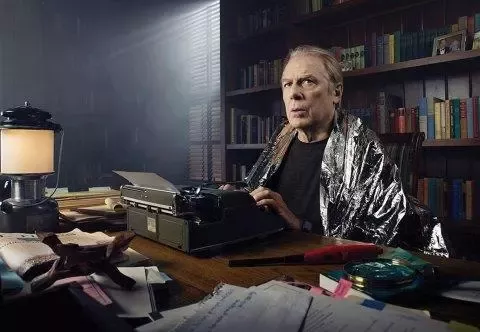
\includegraphics[width=1.6in,height=\textheight]{figuras/chuck.png}

}

\caption{\label{fig-chuck}Chuck McGill fingiendo una enfermedad para
obtener validación de otras personas.}

\end{figure}%

\end{tcolorbox}

\begin{tcolorbox}[enhanced jigsaw, colframe=quarto-callout-important-color-frame, colback=white, colbacktitle=quarto-callout-important-color!10!white, leftrule=.75mm, left=2mm, breakable, coltitle=black, toptitle=1mm, bottomtitle=1mm, rightrule=.15mm, titlerule=0mm, title=\textcolor{quarto-callout-important-color}{\faExclamation}\hspace{0.5em}{Narcisista Encubierto vs.~Narcisista Evidente}, arc=.35mm, bottomrule=.15mm, opacitybacktitle=0.6, opacityback=0, toprule=.15mm]

En la \textbf{Tabla}~\ref{tbl-comparacion}, se presentan las diferencias
clave entre el narcisista encubierto y el narcisista evidente. Mientras
que el narcisista evidente muestra abiertamente su grandiosidad y
necesidad de admiración, el narcisista encubierto lo hace de manera más
sutil, a través de la victimización y la manipulación pasiva.

\begin{longtable}[]{@{}
  >{\raggedright\arraybackslash}p{(\columnwidth - 4\tabcolsep) * \real{0.1341}}
  >{\raggedright\arraybackslash}p{(\columnwidth - 4\tabcolsep) * \real{0.3598}}
  >{\raggedright\arraybackslash}p{(\columnwidth - 4\tabcolsep) * \real{0.5061}}@{}}

\caption{\label{tbl-comparacion}Comparación entre el narcisista
encubierto y el narcisista evidente.}

\tabularnewline

\toprule\noalign{}
\begin{minipage}[b]{\linewidth}\raggedright
Tipo
\end{minipage} & \begin{minipage}[b]{\linewidth}\raggedright
Caracteristicas
\end{minipage} & \begin{minipage}[b]{\linewidth}\raggedright
Ejemplos
\end{minipage} \\
\midrule\noalign{}
\endhead
\bottomrule\noalign{}
\endlastfoot
Narcisista Encubierto & Falsa modestia, victimización, manipulación
pasiva & Chuck McGill (Better Call Saul), `Soy muy brillante, pero el
mundo está contra mí' \\
Narcisista Evidente & Grandiosidad, necesidad de admiración,
manipulación activa & Donald Trump, `Soy el mejor presidente de la
historia, nadie lo hace mejor que yo' \\

\end{longtable}

\end{tcolorbox}

\subsection{Antecedentes}\label{antecedentes}

\begin{tcolorbox}[enhanced jigsaw, colframe=quarto-callout-tip-color-frame, colback=white, colbacktitle=quarto-callout-tip-color!10!white, leftrule=.75mm, left=2mm, breakable, coltitle=black, toptitle=1mm, bottomtitle=1mm, rightrule=.15mm, titlerule=0mm, title=\textcolor{quarto-callout-tip-color}{\faLightbulb}\hspace{0.5em}{Tip}, arc=.35mm, bottomrule=.15mm, opacitybacktitle=0.6, opacityback=0, toprule=.15mm]

\begin{itemize}
\item
  \textbf{Contenido}: Revisión crítica de estudios previos,
  identificando vacíos o contradicciones que tu trabajo abordará.
\item
  \textbf{Estilo narrativo}: Analítico y comparativo. Usa conectores
  como ``Sin embargo\ldots{}'', ``A diferencia de\ldots{}''.
\end{itemize}

\end{tcolorbox}

De acuerdo a \ldots{} (\citeproc{ref-DopaminaYSelfies2019}{González y
Likeador, 2019}; \citeproc{ref-EgoLab2023}{PeerReviewHater y
DataCherryPicker, 2023}).

Sin embargo, los \ac{narc} son peligrosos en la ciencia
(\citeproc{ref-CienciaToxica2024}{Butterfly, 2024};
\citeproc{ref-NeuroFilter2020}{Hashtag, 2020}) ya que estos individuos
suelen:

\begin{itemize}
\tightlist
\item
  Descartar críticas como ``\textbf{envidia académica}''.
\item
  \textbf{Adulterar datos} para que coincidan con su ``brillante
  intuición''.
\item
  \textbf{Desacreditar} colegas con frases como ``Su metodología
  es\ldots{} peculiar'' (traducción: ``Odio que tenga razón'').
\end{itemize}

\subsection{Planteamiento del
problema}\label{planteamiento-del-problema}

\begin{tcolorbox}[enhanced jigsaw, colframe=quarto-callout-tip-color-frame, colback=white, colbacktitle=quarto-callout-tip-color!10!white, leftrule=.75mm, left=2mm, breakable, coltitle=black, toptitle=1mm, bottomtitle=1mm, rightrule=.15mm, titlerule=0mm, title=\textcolor{quarto-callout-tip-color}{\faLightbulb}\hspace{0.5em}{Tip}, arc=.35mm, bottomrule=.15mm, opacitybacktitle=0.6, opacityback=0, toprule=.15mm]

\begin{itemize}
\item
  \textbf{Contenido}: Formula la pregunta de investigación de manera
  clara y específica. Ejemplo: ``¿Cómo afecta la exposición a estrés
  crónico a la neurogénesis en el hipocampo?''.
\item
  Estilo narrativo: Directo y enfocado. Evita ambigüedades.
\item
  Gramática: Usa interrogativas directas o frases declarativas (ej.:
  ``Se desconoce si\ldots{}'').
\end{itemize}

\end{tcolorbox}

\begin{quote}
¿Cómo afecta el narcisismo encubierto a la práctica científica?

¿Es posible hacer ciencia rigurosa cuando tu cerebro interpreta
``revisión por pares'' como ``ataque personal''?
\end{quote}

\begin{quote}
¿Cómo detectar a un narcisista encubierto antes de que te invite a su
monólogo sobre lo ``difícil que es ser tan inteligente y sensible''?
\end{quote}

\subsection{Justificación}\label{justificaciuxf3n}

\begin{tcolorbox}[enhanced jigsaw, colframe=quarto-callout-tip-color-frame, colback=white, colbacktitle=quarto-callout-tip-color!10!white, leftrule=.75mm, left=2mm, breakable, coltitle=black, toptitle=1mm, bottomtitle=1mm, rightrule=.15mm, titlerule=0mm, title=\textcolor{quarto-callout-tip-color}{\faLightbulb}\hspace{0.5em}{Tip}, arc=.35mm, bottomrule=.15mm, opacitybacktitle=0.6, opacityback=0, toprule=.15mm]

\begin{itemize}
\item
  \textbf{Contenido}: Explica por qué el problema es relevante
  científicamente, clínicamente o socialmente. Incluye posibles
  aplicaciones.
\item
  \textbf{Estilo narrativo}: Persuasivo. Destaca el impacto potencial
  (ej.: ``Este estudio podría mejorar estrategias para\ldots{}'').
\end{itemize}

\end{tcolorbox}

Estudiar el \ac{narc} es urgente porque la ciencia no es un monólogo,
pero el narcisista encubierto la trata como su TED Talk personal.
Además, el sesgo de confirmación se vuelve dogma cuando el investigador
cree que ``mi teoría es tan obvia y correcta que hasta mi perro la
entiende''. Por último, hay que evitar que la palabra ``humildad'' sea
secuestrada por narcisistas y salvar a la humanidad de conversaciones
que empiezan con ``Soy demasiado empático y por eso el mundo me odia, es
mi maldición''

\subsection{Objetivos}\label{objetivos}

\begin{tcolorbox}[enhanced jigsaw, colframe=quarto-callout-tip-color-frame, colback=white, colbacktitle=quarto-callout-tip-color!10!white, leftrule=.75mm, left=2mm, breakable, coltitle=black, toptitle=1mm, bottomtitle=1mm, rightrule=.15mm, titlerule=0mm, title=\textcolor{quarto-callout-tip-color}{\faLightbulb}\hspace{0.5em}{Tip}, arc=.35mm, bottomrule=.15mm, opacitybacktitle=0.6, opacityback=0, toprule=.15mm]

\begin{itemize}
\item
  \textbf{Objetivo general}: Amplio y alineado con el problema.
\item
  \textbf{Objetivos específicos}: Medibles y secuenciales.
\item
  \emph{Estilo narrativo}: Imperativo o infinitivo (ej.:
  ``Determinar\ldots{}'', ``Analizar\ldots{}'').
\item
  \emph{Gramática}: Verbos de acción claros (evita ``estudiar'' si es
  vago; usa ``cuantificar'', ``comparar'')
\end{itemize}

\end{tcolorbox}

\begin{enumerate}
\def\labelenumi{\roman{enumi}.}
\item
  Correlacionar puntuaciones de narcisismo encubierto con resistencia a
  la crítica por pares.
\item
  Cuantificar la frecuencia de frases pasivo-agresivas en correos de
  rechazo a colaboradores (``Lamento que no hayas entendido mi
  genialidad'').
\item
  Demostrar que su corteza prefrontal prioriza ``proteger mi ego'' sobre
  ``aceptar evidencia'' mediante fMRI durante discusiones académicas.
\item
  Desarrollar un algoritmo que detecte narcisismo encubierto en reviews
  anónimos (pista: busca la palabra ``claramente'' seguida de un insulto
  o desacreditación).
\item
  Medir la actividad de la dopamina cuando alguien les dice ``Wow, eres
  tan auténtico''.
\end{enumerate}

\subsection{Hipótesis}\label{hipuxf3tesis}

\begin{tcolorbox}[enhanced jigsaw, colframe=quarto-callout-tip-color-frame, colback=white, colbacktitle=quarto-callout-tip-color!10!white, leftrule=.75mm, left=2mm, breakable, coltitle=black, toptitle=1mm, bottomtitle=1mm, rightrule=.15mm, titlerule=0mm, title=\textcolor{quarto-callout-tip-color}{\faLightbulb}\hspace{0.5em}{Tip}, arc=.35mm, bottomrule=.15mm, opacitybacktitle=0.6, opacityback=0, toprule=.15mm]

\begin{itemize}
\item
  \textbf{Contenido}: Propuesta verificable que responde al problema.
  Ejemplo: ``La deprivación de sueño reduce la densidad sináptica en la
  corteza prefrontal''.
\item
  \textbf{Estilo narrativo}: Afirmativo y basado en teoría. Usa
  condicionales si es exploratorio (ej.: ``Se hipotetiza que\ldots{}'').
\item
  \textbf{Gramática}: Presente o futuro simple (ej.: ``Los ratones
  expuestos mostrarán\ldots{}'').
\end{itemize}

\end{tcolorbox}

\begin{tcolorbox}[enhanced jigsaw, colframe=quarto-callout-tip-color-frame, colback=white, colbacktitle=quarto-callout-tip-color!10!white, leftrule=.75mm, left=2mm, breakable, coltitle=black, toptitle=1mm, bottomtitle=1mm, rightrule=.15mm, titlerule=0mm, title=\textcolor{quarto-callout-tip-color}{\faLightbulb}\hspace{0.5em}{Tip}, arc=.35mm, bottomrule=.15mm, opacitybacktitle=0.6, opacityback=0, toprule=.15mm]

NOTA: No formularla como pregunta ni incluir metodología. Es un error
común formular la \textbf{hipótesis} como una \textbf{pregunta} porque,
por definición, una hipótesis es una \textbf{afirmación o proposición}
que se plantea como una posible respuesta a la pregunta de
investigación. La hipótesis no es la pregunta en sí, sino una
\textbf{predicción fundamentada} que se deriva de la teoría y los
antecedentes, y que será sometida a prueba mediante la investigación.

Es muy importante que se formule una hipótesis que pueda ser refutada
(ver
``\href{https://www.scientificamerican.com/article/if-you-say-science-is-right-youre-wrong/}{If
you say Science is Right, you're wrong}'' y
\href{https://es.wikipedia.org/wiki/Falsacionismo}{Falsacionismo}).

\end{tcolorbox}

Proponemos que el narcisista encubierto:

\begin{itemize}
\tightlist
\item
  Distorsiona el método científico para validar su autoimagen,
  convirtiendo hipótesis en horóscopos académicos (``Los datos no
  coinciden, pero mi intuición es un don'').
\item
  Usa la sección de conflicto de intereses para listar enemigos y la
  revisión por pares como método de venganza contra sus enemigos
  (\textbf{\emph{spoiler}}: TODOS son sus enemigos).
\item
  Su actividad cerebral al recibir críticas se asemeja a la de un niño
  viendo arder su jugete en el kindergarten.
\end{itemize}

\subsection{Metodolodía}\label{metodoloduxeda}

\begin{tcolorbox}[enhanced jigsaw, colframe=quarto-callout-tip-color-frame, colback=white, colbacktitle=quarto-callout-tip-color!10!white, leftrule=.75mm, left=2mm, breakable, coltitle=black, toptitle=1mm, bottomtitle=1mm, rightrule=.15mm, titlerule=0mm, title=\textcolor{quarto-callout-tip-color}{\faLightbulb}\hspace{0.5em}{Tip}, arc=.35mm, bottomrule=.15mm, opacitybacktitle=0.6, opacityback=0, toprule=.15mm]

\begin{itemize}
\item
  \textbf{Contenido}: Detalla diseño experimental, sujetos/muestras,
  técnicas (ej.: fMRI, PCR), análisis estadístico y ética.
\item
  \textbf{Estilo narrativo}: Descriptivo y replicable. Usa pasiva para
  objetividad (ej.: ``Se utilizó un diseño doble ciego\ldots{}'').
\item
  \textbf{Gramática}: Pasado si el estudio ya se realizó; presente si es
  una propuesta
\end{itemize}

\end{tcolorbox}

\begin{tcolorbox}[enhanced jigsaw, colframe=quarto-callout-note-color-frame, colback=white, colbacktitle=quarto-callout-note-color!10!white, leftrule=.75mm, left=2mm, breakable, coltitle=black, toptitle=1mm, bottomtitle=1mm, rightrule=.15mm, titlerule=0mm, title=\textcolor{quarto-callout-note-color}{\faInfo}\hspace{0.5em}{Términos Importantes}, arc=.35mm, bottomrule=.15mm, opacitybacktitle=0.6, opacityback=0, toprule=.15mm]

\emph{Metodología}: Este término es más amplio y no solo describe los
procedimientos específicos utilizados en el experimento, sino también
las bases teóricas que justifican esos métodos. Incluye una discusión
sobre por qué ciertos métodos son apropiados para la investigación en
cuestión. Si tu sección describe tanto el ``cómo'' (los pasos y
procedimientos) como el ``por qué'' (la justificación de la elección de
esos métodos).

\emph{Diseño Experimental}: Este término se refiere específicamente al
plan estructural de la investigación, cómo se organizan los
experimentos, qué variables se controlan, cómo se asignan los sujetos a
diferentes grupos, etc. Es más específico que ``Método'' y se centra en
la planificación del experimento en sí.

\emph{Método}: Es un término más específico y directo. Se enfoca en los
pasos concretos y técnicas empleadas en la investigación, sin
necesariamente entrar en detalles sobre la justificación teórica de esos
métodos.

\end{tcolorbox}

\begin{tcolorbox}[enhanced jigsaw, colframe=quarto-callout-caution-color-frame, colback=white, colbacktitle=quarto-callout-caution-color!10!white, leftrule=.75mm, left=2mm, breakable, coltitle=black, toptitle=1mm, bottomtitle=1mm, rightrule=.15mm, titlerule=0mm, title=\textcolor{quarto-callout-caution-color}{\faFire}\hspace{0.5em}{Voz Pasiva en Metodología}, arc=.35mm, bottomrule=.15mm, opacitybacktitle=0.6, opacityback=0, toprule=.15mm]

\emph{Ejemplo de tabla renderizada con Markdown}.

\begin{longtable}[]{@{}
  >{\raggedright\arraybackslash}p{(\columnwidth - 2\tabcolsep) * \real{0.4583}}
  >{\raggedright\arraybackslash}p{(\columnwidth - 2\tabcolsep) * \real{0.5417}}@{}}
\caption{Ejemplos de Voz Activa y Pasiva}\label{tbl-voz}\tabularnewline
\toprule\noalign{}
\begin{minipage}[b]{\linewidth}\raggedright
\textbf{Voz Activa}
\end{minipage} & \begin{minipage}[b]{\linewidth}\raggedright
\textbf{Voz Pasiva}
\end{minipage} \\
\midrule\noalign{}
\endfirsthead
\toprule\noalign{}
\begin{minipage}[b]{\linewidth}\raggedright
\textbf{Voz Activa}
\end{minipage} & \begin{minipage}[b]{\linewidth}\raggedright
\textbf{Voz Pasiva}
\end{minipage} \\
\midrule\noalign{}
\endhead
\bottomrule\noalign{}
\endlastfoot
El presidente pronunció un largo discurso & Un largo discurso fue
pronunciado por el presidente \\
Varios millones visitan Barcelona cada año & Barcelona es visitada cada
año por varios millones \\
Mi madre horneó una tarta de chocolate & Una tarta de chocolate fue
horneada por mi madre \\
Unos ladrones atracaron el banco & El banco fue atracado por unos
ladrone \\
\end{longtable}

\begin{longtable}[]{@{}ll@{}}
\caption{Verbos en Voz Activa y Pasiva}\label{tbl-verbos}\tabularnewline
\toprule\noalign{}
\textbf{Verbo Activo} & \textbf{Verbo Pasivo} \\
\midrule\noalign{}
\endfirsthead
\toprule\noalign{}
\textbf{Verbo Activo} & \textbf{Verbo Pasivo} \\
\midrule\noalign{}
\endhead
\bottomrule\noalign{}
\endlastfoot
Escribe & Es escrito \\
Escribió & Fue escrito \\
Escribirá & Será escrito \\
Escriba & Sea escrito \\
Han escrito & Han sido escritos \\
\end{longtable}

\end{tcolorbox}

\begin{tcolorbox}[enhanced jigsaw, colframe=quarto-callout-tip-color-frame, colback=white, colbacktitle=quarto-callout-tip-color!10!white, leftrule=.75mm, left=2mm, breakable, coltitle=black, toptitle=1mm, bottomtitle=1mm, rightrule=.15mm, titlerule=0mm, title=\textcolor{quarto-callout-tip-color}{\faLightbulb}\hspace{0.5em}{Animales de Laboratorio}, arc=.35mm, bottomrule=.15mm, opacitybacktitle=0.6, opacityback=0, toprule=.15mm]

Reportar el uso de animales de laboratorio, incluyendo:

\begin{itemize}
\tightlist
\item
  Especie, cepa y número de animales
\item
  Cuidado y monitoreo
\item
  Aprovación de comité de ética
\item
  Intervenciones y pasos utilizados para reducir dolor, sufrimiento y
  distrés.
\item
  Cómo se obtuvo el tamaño de la muestra a priori.
\end{itemize}

\end{tcolorbox}

\subsubsection{Disclaimer sobre los sujetos
experimentales}\label{disclaimer-sobre-los-sujetos-experimentales}

Todos los sujetos con personalidad narcisista negaron todos los métodos
y resultados, diciendo ``Yo solo estoy aquí para ayudar a la ciencia''
y/o ``yo haría un mejor estudio'' (clásico).

\subsection{Resultados}\label{resultados}

\subsubsection{Reporte de Animales}\label{reporte-de-animales}

\begin{tcolorbox}[enhanced jigsaw, colframe=quarto-callout-tip-color-frame, colback=white, colbacktitle=quarto-callout-tip-color!10!white, leftrule=.75mm, left=2mm, breakable, coltitle=black, toptitle=1mm, bottomtitle=1mm, rightrule=.15mm, titlerule=0mm, title=\textcolor{quarto-callout-tip-color}{\faLightbulb}\hspace{0.5em}{Tip}, arc=.35mm, bottomrule=.15mm, opacitybacktitle=0.6, opacityback=0, toprule=.15mm]

Contenido: Datos crudos (tablas, gráficos) sin interpretación. Responde
a cada objetivo.

Estilo narrativo: Neutral y factual. Ejemplo: ``El grupo experimental
mostró un 20\% menos de\ldots{}''.

Gramática: Pasado (ej.: ``Se observó una correlación
significativa\ldots{}'').

Resultados vs.~Discusión: No mezclar descripción de datos con
interpretación

\end{tcolorbox}

\subsubsection{Scores de Narcisismo Encubierto correlacionan con rechazo
a
críticas}\label{scores-de-narcisismo-encubierto-correlacionan-con-rechazo-a-cruxedticas}

\todo{ejemplo de gráfico renderizado con R y Datos Simulados en R.}

\begin{verbatim}
[1] "Correlación entre Narcisismo y Rechazo a Críticas: 0.69"
\end{verbatim}

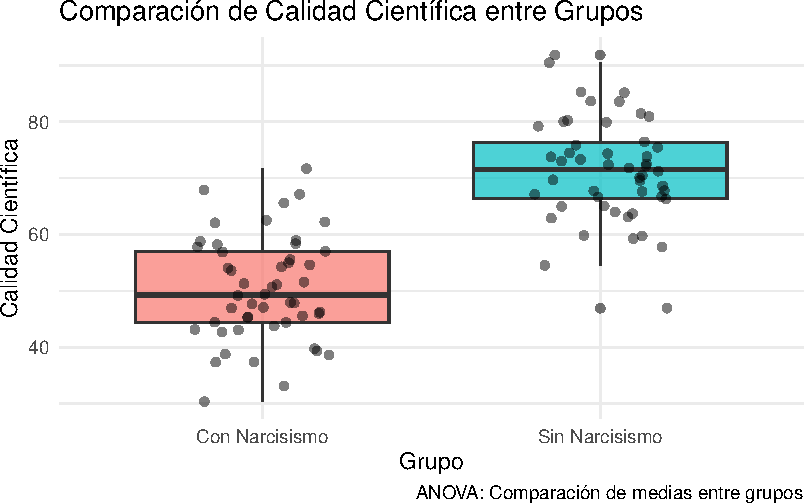
\includegraphics{template_files/figure-pdf/unnamed-chunk-4-1.pdf}

\begin{tcolorbox}[enhanced jigsaw, colframe=quarto-callout-tip-color-frame, colback=white, colbacktitle=quarto-callout-tip-color!10!white, leftrule=.75mm, left=2mm, breakable, coltitle=black, toptitle=1mm, bottomtitle=1mm, rightrule=.15mm, titlerule=0mm, title=\textcolor{quarto-callout-tip-color}{\faLightbulb}\hspace{0.5em}{Tip}, arc=.35mm, bottomrule=.15mm, opacitybacktitle=0.6, opacityback=0, toprule=.15mm]

Puedes usar el paquete de R \texttt{report} (incluido en la app) para
generar automáticamente un informe las pruebas estadísticas en formato
APA. A pesar que por el momento solo lo hace en inglés, te ahorrará
mucho tiempo y asegura calidad y estandarización de tu reporte.

\begin{verbatim}
Effect sizes were labelled following Funder's (2019) recommendations.

The Pearson's product-moment correlation between datos$Narcisismo and
datos$Rechazo_Criticas is positive, statistically significant, and very large
(r = 0.69, 95% CI [0.57, 0.78], t(98) = 9.33, p < .001)
\end{verbatim}

Y luego puedes incluir el resultado en tu texto. \textbf{Esto se hace de
manera automática, por lo que si cambias tus datos, el reporte se
actualiza automáticamente}:

\begin{itemize}
\tightlist
\item
  A mayor narcisismo encubierto, mayor rechazo a críticas constructivas
  (r = 0.69, 95\% CI {[}0.57, 0.78{]}, t(98) = 9.33, p \textless{}
  .001).
\item
  Correlación entre Narcisismo y Rechazo a Críticas: 0.69
\end{itemize}

\end{tcolorbox}

\subsubsection{Activación cerebral en
fMRI}\label{activaciuxf3n-cerebral-en-fmri}

La amígdala se activa un 250\% más al escuchar ``Tu muestra es muy
pequeña'' vs.~``Tu teoría revolucionó la ciencia''.

\begin{Shaded}
\begin{Highlighting}[]
\FunctionTok{install.packages}\NormalTok{(}\StringTok{"fmri"}\NormalTok{)}
\CommentTok{\# devtools::install\_github("muschellij2/fmri")}
\CommentTok{\# https://johnmuschelli.com/Neuroimaging\_in\_R/fmri\_proc.html\#15}
\FunctionTok{library}\NormalTok{(fmri)}

\FunctionTok{source}\NormalTok{(}\StringTok{"https://neuroconductor.org/neurocLite.R"}\NormalTok{)}
\FunctionTok{neuro\_install}\NormalTok{(}\StringTok{"neurobase"}\NormalTok{, }\AttributeTok{release =} \StringTok{"stable"}\NormalTok{)}

\FunctionTok{orthographic}\NormalTok{(data)}
\end{Highlighting}
\end{Shaded}

\subsubsection{Comparación de Calidad Científica entre
Grupos}\label{comparaciuxf3n-de-calidad-cientuxedfica-entre-grupos}

\begin{tcolorbox}[enhanced jigsaw, colframe=quarto-callout-important-color-frame, colback=white, colbacktitle=quarto-callout-important-color!10!white, leftrule=.75mm, left=2mm, breakable, coltitle=black, toptitle=1mm, bottomtitle=1mm, rightrule=.15mm, titlerule=0mm, title=\textcolor{quarto-callout-important-color}{\faExclamation}\hspace{0.5em}{Importante}, arc=.35mm, bottomrule=.15mm, opacitybacktitle=0.6, opacityback=0, toprule=.15mm]

En la app, se incluyen funciones de fórmulas estadísticas para analizar,
graficar y reportar tus datos. Para hacerlo con tus datos, abre el
archivo `./datos/datos.csv' y reemplaza las variables y nombres de
columnas en el código de abajo. Recuerda usar el formato estándar en
ciencia de datos (r, python, spss), el cual corresponde a: una fila por
observación y una columna por variable.

\end{tcolorbox}

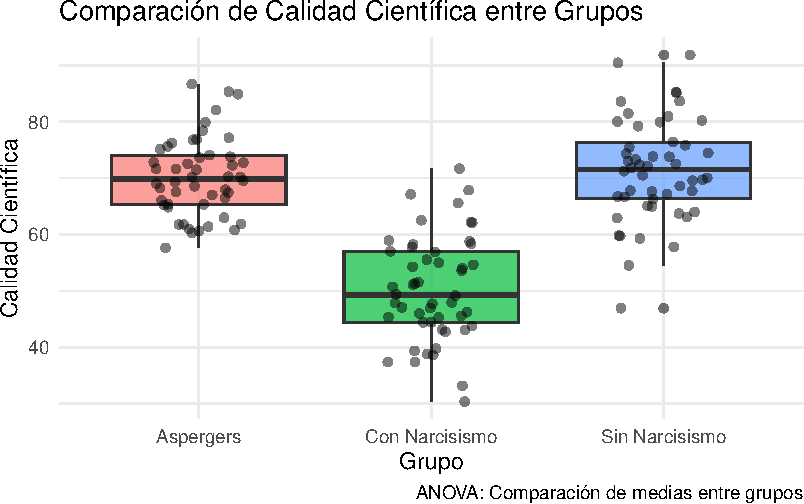
\includegraphics{template_files/figure-pdf/unnamed-chunk-6-1.pdf}

\begin{tcolorbox}[enhanced jigsaw, colframe=quarto-callout-color-frame, arc=.35mm, rightrule=.15mm, colback=white, bottomrule=.15mm, toprule=.15mm, leftrule=.75mm, left=2mm, breakable, opacityback=0]

\vspace{-3mm}\textbf{Funciones Ejemplo para Revisar Supuestos y reportar en formato APA}\vspace{3mm}

\begin{verbatim}

    Shapiro-Wilk normality test

data:  datos_df$calidad_cientifica
W = 0.94834, p-value = 1.309e-06
\end{verbatim}

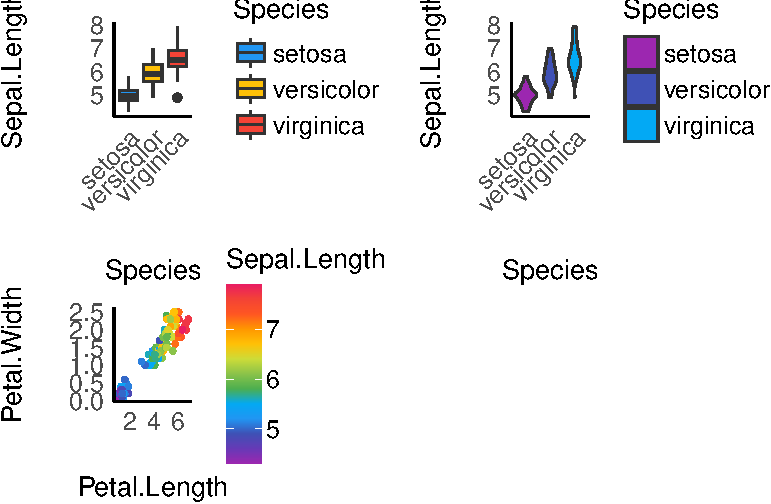
\includegraphics{template_files/figure-pdf/unnamed-chunk-7-1.pdf}

\begin{verbatim}
Effect sizes were labelled following Cohen's (1988) recommendations.

The Welch Two Sample t-test testing the difference of
datos_df$calidad_cientifica by datos_df$personalidad (mean in group narcisista
= 40.12, mean in group otro = 82.94) suggests that the effect is negative,
statistically significant, and large (difference = -42.82, 95% CI [-46.02,
-39.62], t(175.44) = -26.43, p < .001; Cohen's d = -3.74, 95% CI [-4.21,
-3.26])
\end{verbatim}

\end{tcolorbox}

La prueba de T y el gráfico sugieren que las personas con narcisismo
encubierto tienden a tener una calidad científica significativamente
menor\ldots{}
\todo{En discusión, habla mas sobre este resultado y c'omo respalda que el narcisismo encubierto es incompatible con la buena ciencia, ya que afecta negativamente la capacidad de colaborar, aceptar críticas y mantener estándares rigurosos}.

\subsubsection{Más resultados
interesantes}\label{muxe1s-resultados-interesantes}

Más resultados y funciones interesantes para que te inspires. recuerda
que puedes sustituir con tus datos y variables.

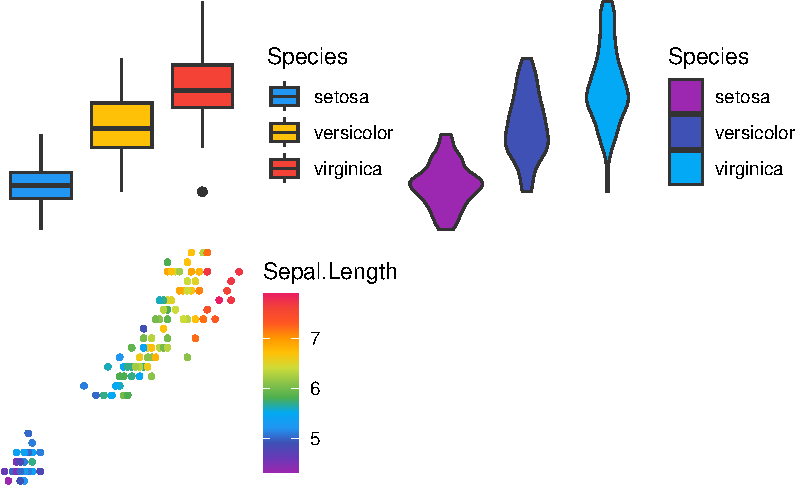
\includegraphics{template_files/figure-pdf/unnamed-chunk-8-1.pdf}

\subsection{Discusión}\label{discusiuxf3n}

\begin{tcolorbox}[enhanced jigsaw, colframe=quarto-callout-tip-color-frame, colback=white, colbacktitle=quarto-callout-tip-color!10!white, leftrule=.75mm, left=2mm, breakable, coltitle=black, toptitle=1mm, bottomtitle=1mm, rightrule=.15mm, titlerule=0mm, title=\textcolor{quarto-callout-tip-color}{\faLightbulb}\hspace{0.5em}{Tip}, arc=.35mm, bottomrule=.15mm, opacitybacktitle=0.6, opacityback=0, toprule=.15mm]

\begin{itemize}
\tightlist
\item
  \textbf{Contenido}: Interpreta resultados, contrasta con antecedentes,
  explica limitaciones y sugiere futuras investigaciones.
\item
  \textbf{Estilo narrativo}: Crítico y reflexivo. Usa comparaciones
  (ej.: ``A diferencia de X, nuestros hallazgos sugieren\ldots{}'').
\item
  \textbf{Gramática}: Presente para teorías aceptadas (ej.: ``Estos
  datos apoyan la hipótesis de que\ldots{}'').
\end{itemize}

\end{tcolorbox}

\subsection{Conclusión}\label{conclusiuxf3n}

\begin{tcolorbox}[enhanced jigsaw, colframe=quarto-callout-tip-color-frame, colback=white, colbacktitle=quarto-callout-tip-color!10!white, leftrule=.75mm, left=2mm, breakable, coltitle=black, toptitle=1mm, bottomtitle=1mm, rightrule=.15mm, titlerule=0mm, title=\textcolor{quarto-callout-tip-color}{\faLightbulb}\hspace{0.5em}{Tip}, arc=.35mm, bottomrule=.15mm, opacitybacktitle=0.6, opacityback=0, toprule=.15mm]

\begin{itemize}
\tightlist
\item
  \textbf{Contenido}: Síntesis de hallazgos clave y su relevancia. No
  repitas resultados.
\item
  \textbf{Estilo narrativo}: Conciso y enfocado en contribuciones.
\item
  \textbf{Gramática}: Presente perfecto o presente (ej.: ``Este estudio
  demuestra que\ldots{}'')
\item
  \textbf{Conclusión}: No introducir nuevos datos o ideas no discutidas
  previamente.
\end{itemize}

\end{tcolorbox}

El narcisismo encubierto es el virus silencioso de la mala ciencia:
convierte la duda en herejía, la colaboración en competencia, y los
journals en diarios íntimos. La solución no es expulsarlos, sino
mandarlos a un retiro espiritual con Alan Watts de fondo (``\emph{The
you who you think you are dpes not exists}'').

\textbf{Propuesta}: incluir tests de narcisismo en las convocatorias de
financiamiento. Cof cof.

Confirmamos que el narcisismo encubierto es como el ajo en las recetas:
todos creen que no lo usan, pero se huele a kilómetros. La neurociencia
sugiere que sus cerebros son máquinas de autoengaño sofisticadas, pero
con suficiente humor y memes, quizá podamos salvarlos (o al menos
reírnos en el proceso). \textbf{Propuesta final}: un bot de Twitter que
responda ``Ok, \emph{Kandel Sebastian Bach}'' a sus hilos existenciales.

\subsection{Apéndices}\label{apuxe9ndices}

\subsubsection{Funciones Extra}\label{funciones-extra}

\begin{tcolorbox}[enhanced jigsaw, colframe=quarto-callout-color-frame, arc=.35mm, rightrule=.15mm, colback=white, bottomrule=.15mm, toprule=.15mm, leftrule=.75mm, left=2mm, breakable, opacityback=0]

Revisar outliers en un modelo de regresión lineal (p.ej., ANOVA).

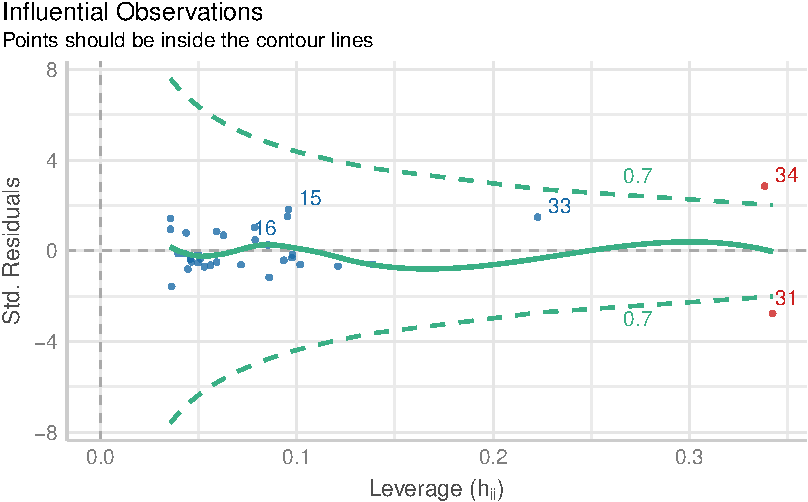
\includegraphics{template_files/figure-pdf/unnamed-chunk-9-1.pdf}

\end{tcolorbox}

\begin{tcolorbox}[enhanced jigsaw, colframe=quarto-callout-color-frame, arc=.35mm, rightrule=.15mm, colback=white, bottomrule=.15mm, toprule=.15mm, leftrule=.75mm, left=2mm, breakable, opacityback=0]

Revisar y Citar paquetes de R utilizados en tu análisis.

\begin{verbatim}
Analyses were conducted using the R Statistical language (version 4.3.1; R Core
Team, 2023) on Ubuntu 22.04.4 LTS, using the packages effectsize (version
0.8.6; Ben-Shachar MS et al., 2020), ggpubr (version 0.6.0; Kassambara A,
2023), parameters (version 0.21.2; Lüdecke D et al., 2020), performance
(version 0.10.7; Lüdecke D et al., 2021), easystats (version 0.6.0; Lüdecke D
et al., 2022), see (version 0.8.0; Lüdecke D et al., 2021), insight (version
0.19.6; Lüdecke D et al., 2019), bayestestR (version 0.13.1; Makowski D et al.,
2019), modelbased (version 0.8.6; Makowski D et al., 2020), report (version
0.5.7; Makowski D et al., 2023), correlation (version 0.8.4; Makowski D et al.,
2022), datawizard (version 0.9.0; Patil I et al., 2022), ggplot2 (version
3.4.4; Wickham H, 2016) and dplyr (version 1.1.3; Wickham H et al., 2023).

References
----------
  - Ben-Shachar MS, Lüdecke D, Makowski D (2020). "effectsize: Estimation of
Effect Size Indices and Standardized Parameters." _Journal of Open Source
Software_, *5*(56), 2815. doi:10.21105/joss.02815
<https://doi.org/10.21105/joss.02815>, <https://doi.org/10.21105/joss.02815>.
  - Kassambara A (2023). _ggpubr: 'ggplot2' Based Publication Ready Plots_. R
package version 0.6.0, <https://rpkgs.datanovia.com/ggpubr/>.
  - Lüdecke D, Ben-Shachar M, Patil I, Makowski D (2020). "Extracting, Computing
and Exploring the Parameters of Statistical Models using R." _Journal of Open
Source Software_, *5*(53), 2445. doi:10.21105/joss.02445
<https://doi.org/10.21105/joss.02445>.
  - Lüdecke D, Ben-Shachar M, Patil I, Waggoner P, Makowski D (2021).
"performance: An R Package for Assessment, Comparison and Testing of
Statistical Models." _Journal of Open Source Software_, *6*(60), 3139.
doi:10.21105/joss.03139 <https://doi.org/10.21105/joss.03139>.
  - Lüdecke D, Ben-Shachar M, Patil I, Wiernik B, Makowski D (2022). "easystats:
Framework for Easy Statistical Modeling, Visualization, and Reporting." _CRAN_.
R package, <https://easystats.github.io/easystats/>.
  - Lüdecke D, Patil I, Ben-Shachar M, Wiernik B, Waggoner P, Makowski D (2021).
"see: An R Package for Visualizing Statistical Models." _Journal of Open Source
Software_, *6*(64), 3393. doi:10.21105/joss.03393
<https://doi.org/10.21105/joss.03393>.
  - Lüdecke D, Waggoner P, Makowski D (2019). "insight: A Unified Interface to
Access Information from Model Objects in R." _Journal of Open Source Software_,
*4*(38), 1412. doi:10.21105/joss.01412 <https://doi.org/10.21105/joss.01412>.
  - Makowski D, Ben-Shachar M, Lüdecke D (2019). "bayestestR: Describing Effects
and their Uncertainty, Existence and Significance within the Bayesian
Framework." _Journal of Open Source Software_, *4*(40), 1541.
doi:10.21105/joss.01541 <https://doi.org/10.21105/joss.01541>,
<https://joss.theoj.org/papers/10.21105/joss.01541>.
  - Makowski D, Ben-Shachar M, Patil I, Lüdecke D (2020). "Estimation of
Model-Based Predictions, Contrasts and Means." _CRAN_.
<https://github.com/easystats/modelbased>.
  - Makowski D, Lüdecke D, Patil I, Thériault R, Ben-Shachar M, Wiernik B (2023).
"Automated Results Reporting as a Practical Tool to Improve Reproducibility and
Methodological Best Practices Adoption." _CRAN_.
<https://easystats.github.io/report/>.
  - Makowski D, Wiernik B, Patil I, Lüdecke D, Ben-Shachar M (2022).
"correlation: Methods for Correlation Analysis." Version 0.8.3,
<https://CRAN.R-project.org/package=correlation>. Makowski D, Ben-Shachar M,
Patil I, Lüdecke D (2020). "Methods and Algorithms for Correlation Analysis in
R." _Journal of Open Source Software_, *5*(51), 2306. doi:10.21105/joss.02306
<https://doi.org/10.21105/joss.02306>,
<https://joss.theoj.org/papers/10.21105/joss.02306>.
  - Patil I, Makowski D, Ben-Shachar M, Wiernik B, Bacher E, Lüdecke D (2022).
"datawizard: An R Package for Easy Data Preparation and Statistical
Transformations." _Journal of Open Source Software_, *7*(78), 4684.
doi:10.21105/joss.04684 <https://doi.org/10.21105/joss.04684>.
  - R Core Team (2023). _R: A Language and Environment for Statistical
Computing_. R Foundation for Statistical Computing, Vienna, Austria.
<https://www.R-project.org/>.
  - Wickham H (2016). _ggplot2: Elegant Graphics for Data Analysis_.
Springer-Verlag New York. ISBN 978-3-319-24277-4,
<https://ggplot2.tidyverse.org>.
  - Wickham H, François R, Henry L, Müller K, Vaughan D (2023). _dplyr: A Grammar
of Data Manipulation_. https://dplyr.tidyverse.org,
https://github.com/tidyverse/dplyr.
\end{verbatim}

\end{tcolorbox}

\subsection{Agradecimientos}\label{agradecimientos}

Cada participante con personalidad Narcisista que colaboró en este
estudio, sin saberlo, merece un agradecimiento especial. Agradecemos a
la Dra. Narcissus por su supervisión y a los Drs. Socrates y Plato por
sus valiosas sugerencias. Agradecemos a la Facultad de Thespiae in
Boeotia por su apoyo financiero y a la Academia of Athens por su
infraestructura.

Finalmente, los participantes con personalidad narcisista pidieron ser
mencionados en los créditos como ``\emph{los verdaderos héroes de la
ciencia}'' o ``\emph{los únicos que entienden la verdadera ciencia}''.

\subsection*{Referencias}\label{referencias}
\addcontentsline{toc}{subsection}{Referencias}

\phantomsection\label{refs}
\begin{CSLReferences}{1}{0}
\bibitem[\citeproctext]{ref-CienciaToxica2024}
Butterfly, Dr. I. R. (2024). \emph{Ciencia Tóxica: Cuando el Ego es el
Principal {COI} (Conflicto de Intereses)}. Cambridge: Black Hole
Academic Press.

\bibitem[\citeproctext]{ref-First2013}
First, M. B. (2013). Diagnostic and Statistical Manual of Mental
Disorders, 5th Edition, and Clinical Utility. \emph{Journal of Nervous
\& Mental Disease}, \emph{201}(9), 727-729.
\url{https://doi.org/10.1097/nmd.0b013e3182a2168a}

\bibitem[\citeproctext]{ref-DopaminaYSelfies2019}
González, D., y Likeador, S. (2019). La Curva de la Dopamina en
Publicaciones de Café Artesanal: Un Estudio con Narcisistas Encubiertos.
\emph{Annual Review of Pretentious Behavior}, \emph{7}, 42-666.
\url{https://doi.org/10.6666/ar.pb.2019.007}

\bibitem[\citeproctext]{ref-NeuroFilter2020}
Hashtag, A. (2020). NeuroFilter: Cómo Detectar un {{«Humblebrag»}} en
280 Caracteres o Menos. En T. Académico (Ed.), \emph{Memes y Neuronas:
La Ciencia detrás de tu Timeline Tóxico} (pp. 69-420). TikTok Academic
Publications.

\bibitem[\citeproctext]{ref-EgoLab2023}
PeerReviewHater, R., y DataCherryPicker, E. (2023). Narcissus in the
Lab: How Covert Narcissism Corrupts Citation Networks. \emph{Journal of
Irreproducible Results}, \emph{12}, 45-69.
\url{https://doi.org/10.6666/jir.2023.045}

\bibitem[\citeproctext]{ref-AlgorithmShade2024}
Sarcasmo, A. (2024). \emph{Detecting Academic Narcissism via
Passive-Aggressive LaTeX Comments: A Machine Learning Approach}
(Technical Report N.º IDPR-666). Recuperado de Institute of Dramatic
Peer Review website: \url{https://arxiv.org/abs/2404.01joke}

\end{CSLReferences}



\end{document}
